\chapter{Firewall}

The goals of this assignment are the following.

\begin{itemize}
\item Familiarizing ourselves with firewalls.
\item Correctly configuring the different options.
\item Configuring a local area network, establishing different security polices using filtering and traffic monitoring.
\item Solve a case study about connecting a Small/Medium Enterprise (SME) network to the Internet using a firewall.
\end{itemize}

\section{Home Preparation}

The Cisco firewall can be configured using a Java program which is called \emph{Adaptive Security Device Manager} (ASDM). This tool makes it possible to interact with the firewall using a graphical user interface (GUI) on a computer with the Windows operating system.

Read more from the following document:
\url{www.jaumebarcelo.info/teaching/lxs/ipsec/ASA_Getting_Started.pdf}
Read also all the assignment and prepare a solution for the \emph{case study}.

You can download a copy of the Cisco ASDM software from the following link.
\url{https://www.dropbox.com/s/5yjqflzvgrlere0/asa.zip}

In the beginning, we can familiarize ourselves with the Adaptive Security Device Manager (ASDM) software using a demo version. The software requires the Java Runtime Environment (JRE) version 1.6.18. After installing and launching the program, select the {\sf Run in Demo Mode} checkbox and choose the desired demo version. The version we use during this practice is 5.2.


\section{Configuring the working place}

For this practical exercise, each group needs 3 computers and a Cisco ASA 5505 firewall. Connect one of the computers to switch B via the patch panel. Before disconnecting this computer from the Internet, download an FTP server such as \emph{Filezilla}. Connect the other two computers to the two internal ports of the firewall (ports 2 and 3).

Connect the firewall to the switch B via the patch panel. Configure the IP address on the external interface (\emph{outside}) of the firewall according to the figure \ref{fig:Firewall}, where \emph{X} is the number of your group. Configure the default gateway of the three computers with the IP address of the corresponding firewall interface, internal (\emph{inside}) for the internal computers and external (\emph{outside}) for the external computers.

\begin{figure}
\centering
\ifpdf
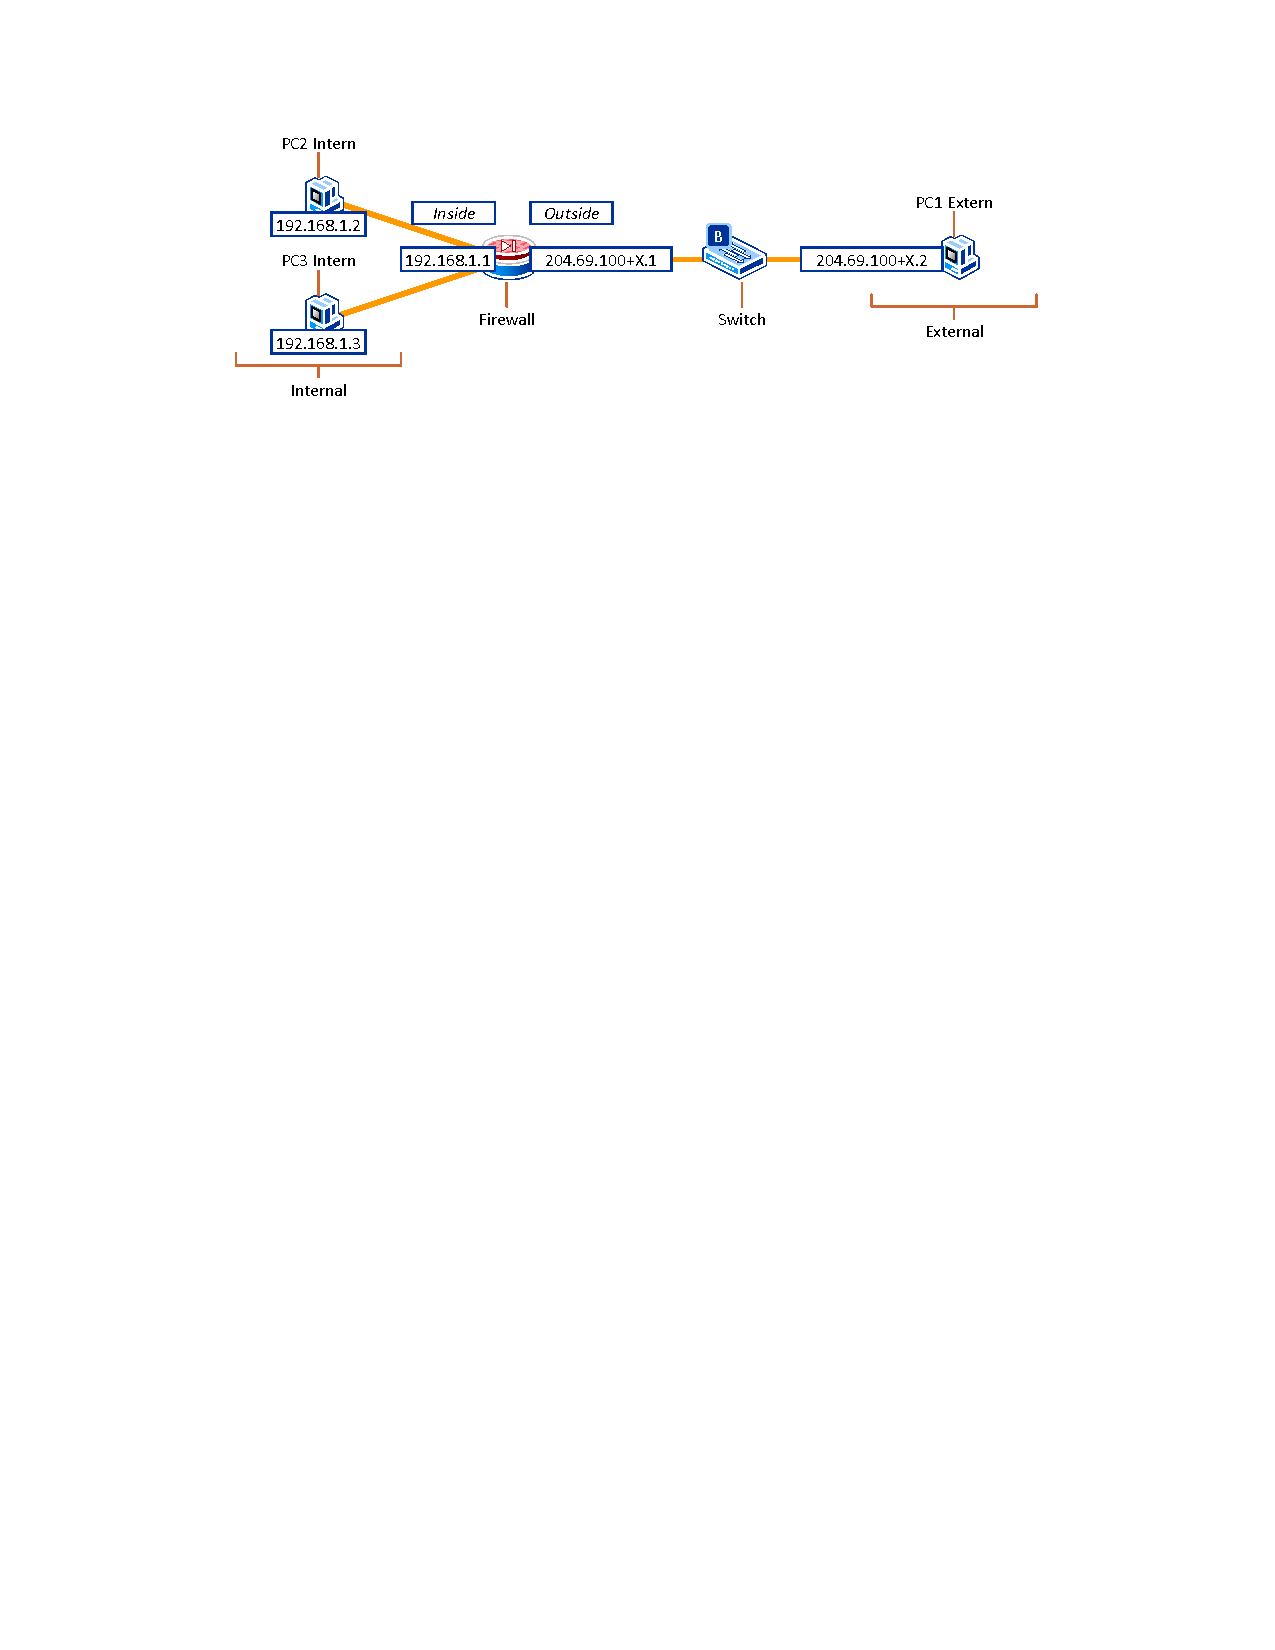
\includegraphics[width=0.9\linewidth]{Figures/Firewall.pdf}
\else
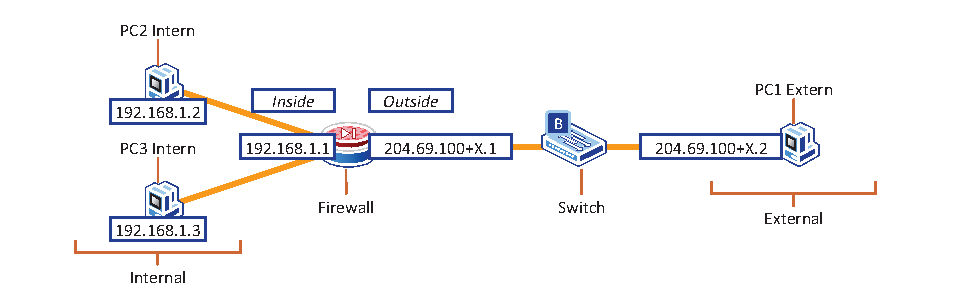
\includegraphics[width=0.9\linewidth]{Figures/Firewall.eps}
\fi
\caption{The network topology for the firewall lab assignment.}
\label{fig:Firewall}
\end{figure}

We shall use the FTP to verify that our network configuration works. Identify the transport layer protocol and the port number for FTP.

\section{Adaptive Security Device Manager (ASDM)}

We will find the \emph{ASMD launcher} on the desktop. The default username and password are blank. The default IP address of the firewall is 192.168.1.1 .

The CISCO ASA firewalls assign a \emph{security level} to the interfaces. A security level of 100 means the interface is 100\% trusted. A security level of 0 means that the interface is not trusted at all. We shall check the interfaces available and their security level. Discuss the appropriateness of this configuration.

We try to ping between the two computers connected to the internal interfaces.

\begin{center}
\sffamily\small
\begin{tabular}{>{\columncolor{tablegray}}p{15cm}}
\multicolumn{1}{>{\columncolor{tableorange}}l}{Question}\\
Does it work? Why?\\
\hline
\end{tabular}
\end{center}

\section{Default Configuration of the ASA 5505}

The Cisco ASA use the same OS that the other devices used in the previous assignments, the Cisco IOS. Open the \textsf{Options} \textgreater \textsf{Preferences} menu and check the \textsf{Preview commands before sending them to the device} option. This will show us the equivalent commands that would be used on the console to change the configuration.

Explain which is the default configuration of the firewall. Observe and explain the different aspects that can be configured using the icons on the left hand side of the screen.

\begin{center}
\sffamily\small
\begin{tabular}{>{\columncolor{tablegray}}p{15cm}}
\multicolumn{1}{>{\columncolor{tableorange}}l}{Questions}\\
What is the default configuration of Ethernet 0/0 (outside)?\\
\hline
Why do you thing that the router ships with this configuration?\\
\hline
\end{tabular}
\end{center}

Now, we will change the IP address of the Ethernet 0/0 (\emph{outside}) interface to 204.69.100+X.1. Remember that the X is the group number, and use a /24 network mask. Now we connect the external computer (via switch B) to the \emph{outside} interface. We configure the IP of the external computer to an address of the outside range and we set the firewall's outside address as the computer's default gateway.

\begin{center}
\sffamily\small
\begin{tabular}{>{\columncolor{tablegray}}p{15cm}}
\multicolumn{1}{>{\columncolor{tableorange}}l}{Questions}\\
Can you ping from the outside PC to an inside PC? Why?\\
\hline
What is the difference compared to the previous case?\\
\hline
\end{tabular}
\end{center}

Look at the \textsf{Syslog} from the \textsf{Home} screen to answer this questions.

\section{Firewall}

An alternative configuration option is Telnet. We can enable the Telnet options from the ASDM configuration page using \textsf{Properties} \textgreater \textsf{Device Access} \textgreater \textsf{Telnet}. We have to make sure that we have applied the changes.
Now we connect to the device using a Telnet client and \texttt{cisco} (small letters) as a password.

We try the
\begin{lstlisting}
# who
\end{lstlisting}
command to see who is connected to the firewall.
\begin{lstlisting}
# show run
\end{lstlisting}
to see the running configuration.
Find information about Telnet and DHCP and explain it.
We also try the commands
\begin{lstlisting}
# show interface
\end{lstlisting}
and
\begin{lstlisting}
# show traffic
\end{lstlisting}
and explain the information that they provide.

Discuss the security implications of connecting using Telnet of the console.

\section{The Hosts/Networks Table}

In the \textsf{Network Objects/Groups} tab (from the \textsf{Configuration} \textgreater \textsf{Global Objects} page) we can view, edit, add and delete hosts and networks lists defined for every interface. The hosts and networks are organized according to the interface they are connected to (inside/outside). It is recommended to name all the hosts we are managing.

We add the two internal computers by selecting \textsf{Add} \textgreater \textsf{Network Object...}. The network mask is 255.255.255.255, as it is a single host. Add also a corresponding object for the external computer. We apply to save the changes.

\section{Access Rules}

The access rules make it possible to establish security policies as a list of rules. The tables to specify how a computer interacts with another by allowing and denying specific services and protocols. We try to connect from the inside computer to the outside computer and explain the behavior and the default \textsf{Access Rules} (from the \textsf{Configuration} \textgreater \textsf{Security Polivy} page) table for the inside interface.

The rules are examined sequentially until one of the applies. If the first rule applies, the second is not checked. If the first rule does not apply, then the second is checked. The process is repeated until one of the rules applies.

\begin{center}
\sffamily\small
\begin{tabular}{>{\columncolor{tablegray}}p{15cm}}
\multicolumn{1}{>{\columncolor{tableorange}}l}{Question}\\
The last rule is \emph{any to any deny}. Why?\\
\hline
\end{tabular}
\end{center}

The first rule allows traffic from any IP source to any IP destination if the destination interface has a lower security level. If this rule does not apply, the second rule is examined. The second rule always applies and discards the packet.

We shall observe and explain the rules for the traffic arriving to the external interfaces. To understand the rules, we will pay attention to the graphical diagrams offered by the software.`

We shall install and configure the FTP server to the external computer. Remember that it is needed to add a folder.

\begin{center}
\sffamily\small
\begin{tabular}{>{\columncolor{tablegray}}p{15cm}}
\multicolumn{1}{>{\columncolor{tableorange}}l}{Question}\\
Is it possible to access the FTP server from the internal computers?\\
\hline
\end{tabular}
\end{center}

Use the rules to deny the access to the FTP server to one of the internal computers and allow access to the other. Observe the log messages to verify that access is being denied. Each time that you change the configuration and try to access to the ftp server, clean the browser cache.

\section{Translation Rules}

The ASA 5505 supports both network address translation (NAT) which is a one-to-one address translation (one inside to one outside) and port address translation (PAT) which is a many-to-one address translation. Look at the default configuration for the translation rules.

\begin{center}
\sffamily\small
\begin{tabular}{>{\columncolor{tablegray}}p{15cm}}
\multicolumn{1}{>{\columncolor{tableorange}}l}{Questions}\\
How does this configuration affect outgoing traffic?\\
\hline
What is the IP address used after the packets traverse the firewall?\\
\hline
\end{tabular}
\end{center}

\section{Monitoring}

We can use the ASDM for network monitoring. It allows to select the message supervising level. Check the Telnet connections and connected users using the options of the menu on the left. There is also a tool to generate graphs such as traffic, memory and CPU. Look at some of the graphs and enumerate them.

\section{Case Study}

An enterprize has a C class network 204.69.100+X.0 and wants securely connect their internal network to an external network. The address of the outside firewall interface is 204.69.100+X.1.

In the internal network there is an FTP server with address 192.168.1.4 that needs to be accessed from the outside network using the address 204.69.100+X.4.

The other requirements are that internal users must be able to ping external devices, but not the other way around.

We shall configure the firewall to satisfy the above requirements. Explain the changes that we have made and the tests performed to verify the correctness of the configuration.
